\chapter*{Microphone calibration software} \label{appendix:calibration}
In this appendix the microphone calibration software will be briefly explained. The gold of this software is to be able to calibrate any microphone including the calibration of the soundcard in MATLAB, such that a calibration tone correspond to a known digital number in MATLAB. 

\section*{Materials and setup}
To do a calibration of a random microphone, the following materials are used:
\begin{itemize}
\item RME FIREFACE UCX (Soundcard)
\begin{itemize}[noitemsep]
\item AAU-number: 108230
\item Serial number: 23811948
\end{itemize}
\item E.g. \gls{bandk} TYPE 4231 (calibrator )
\begin{itemize}[noitemsep]
\item AAU-number: 33691
\item Serial number: 2115338
\end{itemize}
\item MATLAB 2017b (PC - software)
\item Random microphone 
\item XLR signal cable
\end{itemize}


\paragraph{The first step}

\begin{figure}[H]
\centering
\begin{picture}(0,0)%
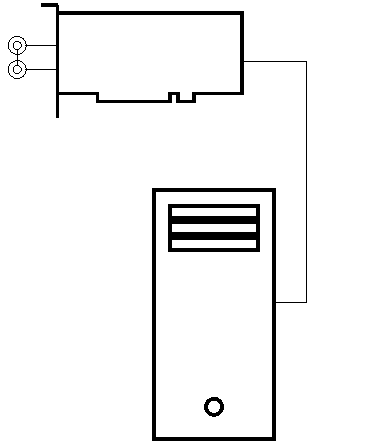
\includegraphics{rme_transfer_function.pdf}%
\end{picture}%
\setlength{\unitlength}{2818sp}%
%
\begingroup\makeatletter\ifx\SetFigFont\undefined%
\gdef\SetFigFont#1#2#3#4#5{%
  \reset@font\fontsize{#1}{#2pt}%
  \fontfamily{#3}\fontseries{#4}\fontshape{#5}%
  \selectfont}%
\fi\endgroup%
\begin{picture}(4090,4926)(8176,-7474)
\put(8191,-3661){Out}%
\put(9271,-3211){Sound Card}%
\put(9971,-6361){Computer}%
\put(11836,-4696){USB}%
\put(8281,-2806){In}%
\end{picture}%
\caption{Setup for calibrating the soundcard}
		\label{fig:appendix:rme_calibration}
\end{figure}

\paragraph{The second step}

\begin{figure}[H]
\centering
\begin{picture}(0,0)%
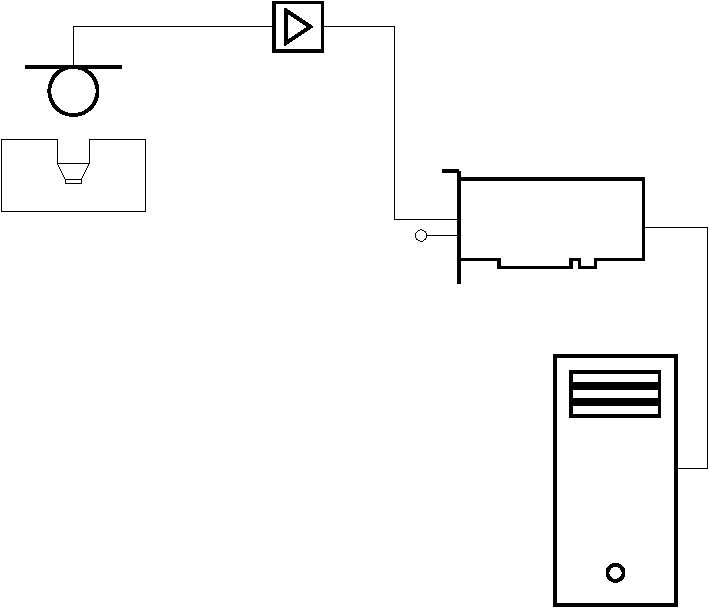
\includegraphics{mic_calibration.pdf}%
\end{picture}%
\setlength{\unitlength}{2818sp}%
%
\begingroup\makeatletter\ifx\SetFigFont\undefined%
\gdef\SetFigFont#1#2#3#4#5{%
  \reset@font\fontsize{#1}{#2pt}%
  \fontfamily{#3}\fontseries{#4}\fontshape{#5}%
  \selectfont}%
\fi\endgroup%
\begin{picture}(7944,6816)(3679,-7474)
\put(10036,-6361){Computer}%
\put(4951,-1771){Microphone}%
\put(6661,-1501){Amplifier}%
\put(9271,-3211){Sound Card}%
\put(8171,-3096){In}%
\put(8171,-3626){Out}%
\put(3961,-2941){Calibrator}%
\put(11746,-4606){USB}%
\end{picture}%
\caption{Setup for calibrating the microphone}
		\label{fig:appendix:mic_calibration}
\end{figure}

\section*{The calibration step} \label{apendix:calibrate_sound_card_and_microphone}
\paragraph{The first step} is measuring the transfer function of the sound card according to \autoref{Frequency_response_of_RME_FIREFACE_UCX} and the set up is shown is \autoref{fig:appendix:rme_calibration}. The complex transfer function is divided by the input of the sound card, such that the gain between input and output of the sound card is 1 from \SI{20}{\hertz} to \SI{20}{\kilo\hertz}, when a signal cable is connected between input and output. While doing the calibration, the peak value at the input is saved and used as a reference value of the sound card. All measurement have to include the calibration of the sound card, to ensure that a known digital number in MATLAB correspond to a known pressure.
\paragraph{The second step} is measuring the digital number in MATLAB that corresponding to \SI{1}{\pascal} or \SI{94}{\decibel} and then log value as the microphone calibration peak value. The set up is shown is \autoref{fig:appendix:mic_calibration}. The factor between reference value of the sound card divided by the microphone calibration correspond to the factor that have to be multiplied to the input of the sound card, and only works with the microphone used in the calibration. This calibration have to be done before every series of measurement. The function will return the digital number 1 when the pressure is \SI{1}{\pascal} and is linearly depending on the pressure. To calculate the \gls{spl} the following formula is used

\begin{equation}
dB\,\, re. \SI{20}{\micro\pascal} = 20 \cdot log_{10} \left ( \frac{p}{p_0} \right )
\end{equation}

    \startexplain
    		\explain{$p$ is the returned number from the function }{\si{\pascal}}
        \explain{$p_0$ is the reference pressure}{\si{\pascal}}
    \stopexplain  


\section*{The MATLAB function for measuring the input}
To ensure that the calibration and measuring record software is as identical as possible, the same function is used just modified so instead of playing a swept sine, it will play a string of zero.

\section*{The MATLAB function}
\includeCode{irmeas_fft_mic.m}{matlab}{1}{40}{The calibration record software}{code:irmeas_fft_mic}{./code/microphone_calibration/sine_sweep/}



